\documentclass{article}
\usepackage[colorlinks=true, allcolors=blue]{hyperref}
\usepackage{tabularray}
\usepackage{amssymb}
\usepackage{graphicx} % Required for inserting images

\title{Results}
\author{Automatic Project Detection And Tooling For Devs}
\date{}

\begin{document}
\maketitle

\clearpage

\section{Marketing}

We have created a marketing poster with the team, showcasing the main pages of our software. Alongside this, we also produced a video that highlights the key features and demonstrates how to use them effectively. Both the poster and the video aim to provide a clear and engaging overview of our software, helping potential users to understand its capabilities and benefits.

\subsection{Marketing poster}
The poster is available on \href{https://github.com/CsullogBeni/szofttech/blob/main/documentation/img/poster.png}{github},
\begin{figure}[h!]
    \centering
    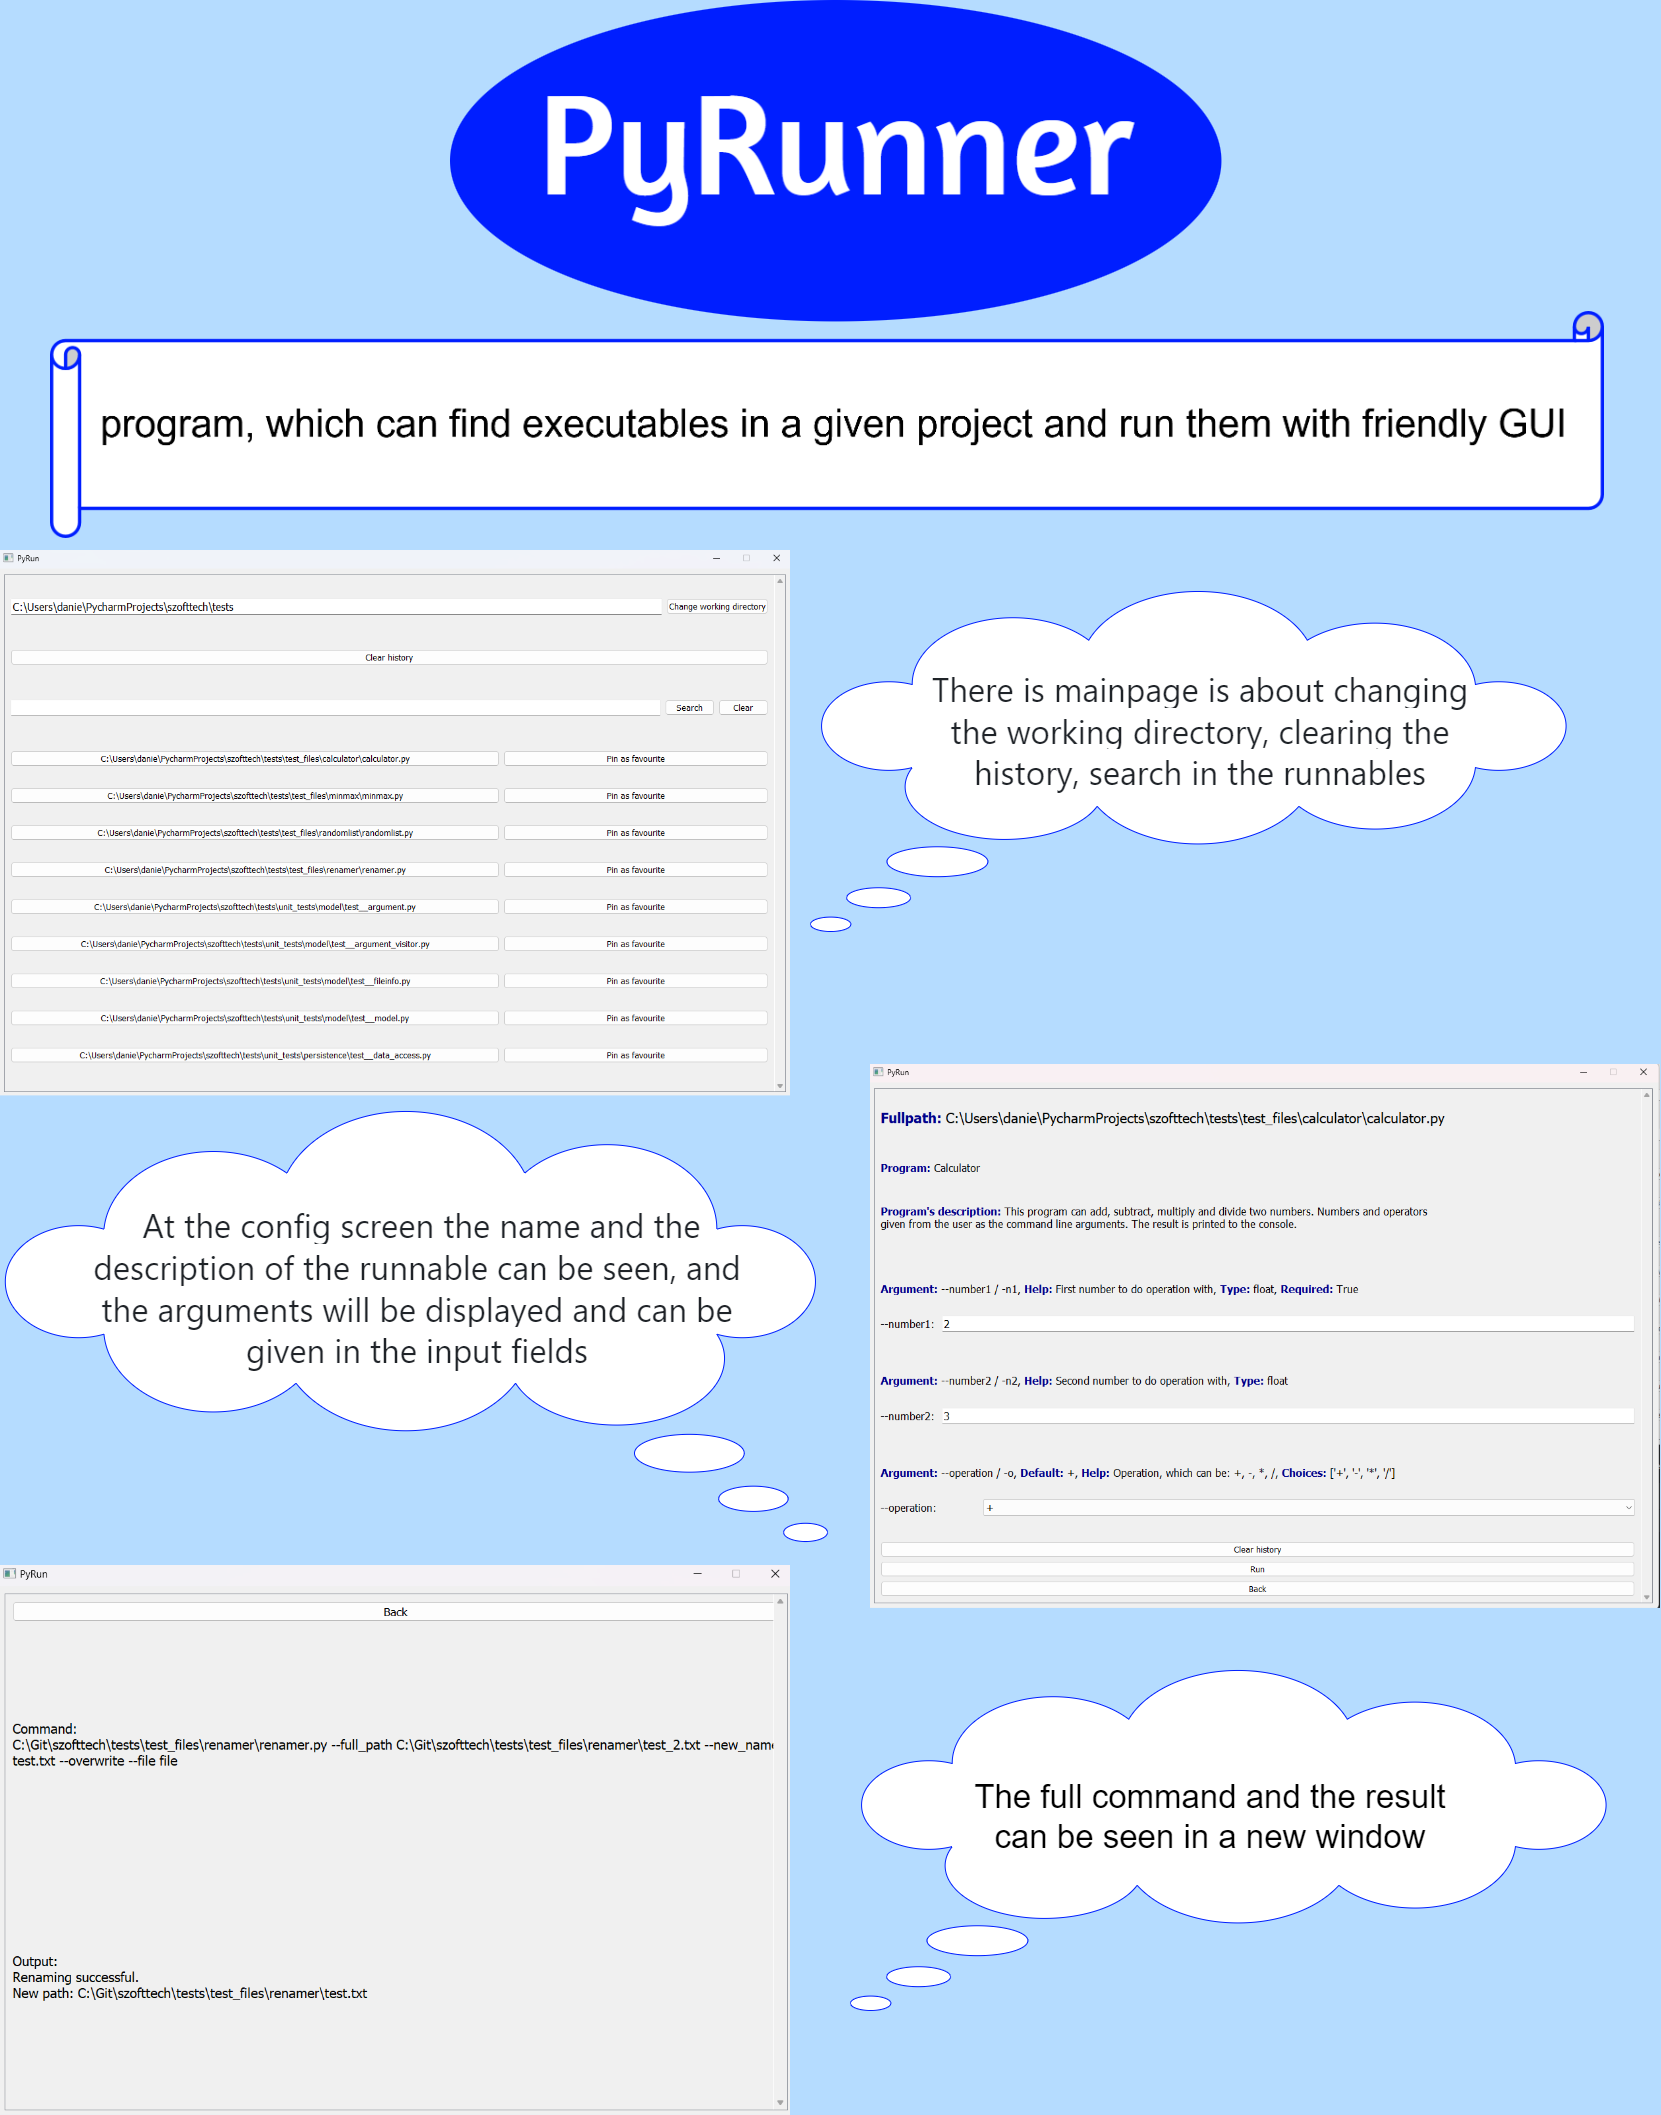
\includegraphics[width=0.8\linewidth]{img/poster.png}
    \caption{Marketing poster}
    \label{fig:enter-label}
\end{figure}

\subsection{Marketing video}

The video is available on \href{https://github.com/CsullogBeni/szofttech/tree/main/documentation/video}{github}.

\subsection{Software requirements}

The following tools and environments are required:

\begin{itemize}
    \item Operating System\@: Windows/Linux/MacOS
    \item Programming Language\@: Node.js or Python (v3.8+)
    \item Additional dependencies\@: PyQt5
    \item Disk space\@: At least 500MB of free space
    \item RAM\@: 4GB minimum (recommended 8GB for better performance)
\end{itemize}

\section{Software installation}

To install the software, follow these steps:

\begin{enumerate}
    \item Open a command line prompt, where you want to install your software
    \item Clone the repository\@: \texttt{git clone https://github.com/CsullogBeni/szofttech.git}.
    \item Activate conda environment or download Python v3.8 or higher
    \item Install dependencies\@: Run \texttt{pip install PyQt5}
    \item Set python path: \texttt{set PYTHONPATH=<Full path to the directory that contains the project>}
    \item Start the application from a command line prompt. Navigate to the directory that contains the project. Run: \@\texttt{python ./src/view/main.py}.
\end{enumerate}

\section{Project tools}

\subsection{Version Control System}

Throughout the development process, we utilized Git as our version control system and hosted the project on GitHub. The entire project, including tasks, pull requests, documentation, and a detailed README file, is available there. You'll also find various marketing materials, brainstorming notes, and ideas shared during the project. This comprehensive repository reflects both the technical and creative efforts behind our work, making it a valuable resource for anyone interested in exploring the project's details.

Useful links to the project:
\begin{itemize}
    \item Github that contains the whole project: \href{https://github.com/CsullogBeni/szofttech}{https://github.com/CsullogBeni/szofttech}
    \item Documentation that contains the User, MVP, Plan, Retrospective and results: \href{https://github.com/CsullogBeni/szofttech/tree/main/documentation}{https://github.com/CsullogBeni/szofttech/tree/main/documentation}
    \item Here are all the tasks throughout the project: \href{https://github.com/CsullogBeni/szofttech/issues?q=}{https://github.com/CsullogBeni/szofttech/issues?q=}
    \item All the pull requests that are made: \href{https://github.com/CsullogBeni/szofttech/pulls?q=}{https://github.com/CsullogBeni/szofttech/pulls?q=}
    \item You can find here the directory that contains all the source files that are implemented: \href{https://github.com/CsullogBeni/szofttech/tree/main/src}{https://github.com/CsullogBeni/szofttech/tree/main/src}
    %\item We implemented unit test and system test files for the project: \href{https://github.com/CsullogBeni/szofttech/tree/main/tests/unit_tests}{https://github.com/CsullogBeni/szofttech/tree/main/tests/unit_tests}
    %\item Also We have created a code base that contains many runnable scripts, and we have tested our program on these: \href{https://github.com/CsullogBeni/szofttech/tree/main/tests/test_files}{https://github.com/CsullogBeni/szofttech/tree/main/tests/test_files}
    \item We made a few discussions as well: \href{https://github.com/CsullogBeni/szofttech/discussions}{https://github.com/CsullogBeni/szofttech/discussions}
\end{itemize}

\section{Completed MVP parts}

\begin{figure}[h]
    \centering
    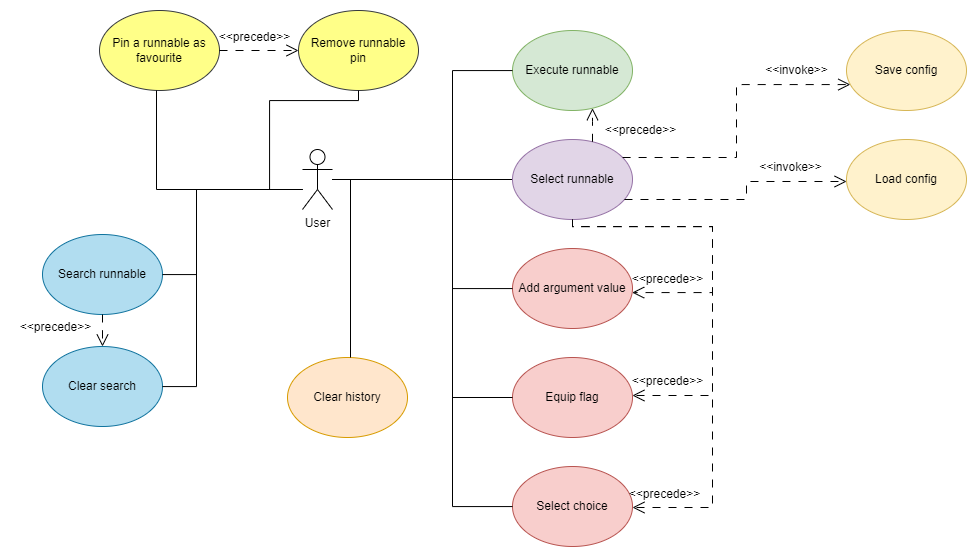
\includegraphics[width=1\linewidth]{img/use_case_diagram.drawio.png}
    \caption{Use case diagram}
    \label{fig:enter-label}
\end{figure}

\subsection{Content of the MVP}
Here are the \href{https://github.com/CsullogBeni/szofttech/blob/main/documentation/mvp.pdf}{MVP} points that We have fulfilled:
\begin{itemize}
    \item Select executable
    \item Add values to arguments
    \item Toggle flag
    \item Select choices
    \item Execute program
    \item Save config
    \item Load config
    \item Clear history
    \item Search executable
    \item Clear search
    \item Pin an executable
    \item Unpin an executable
\end{itemize}

\subsection{MVP parts in the program}

After the program initialization, on the main page:
\begin{itemize}
    \item The Users are able to set the current working directory.
    \item Users are also be able to set their configuration history.
    \item The Users can search for their runnable scripts from the working directory.
    \item They can also clear their search.
    \item On the main page all the pinned runnable files are shown first.
    \item After the pinned ones, there are all the other scripts.
    \item Next to the runnable button the Users can set the pinned status of a script.
\end{itemize}

\begin{figure}[h]
    \centering
    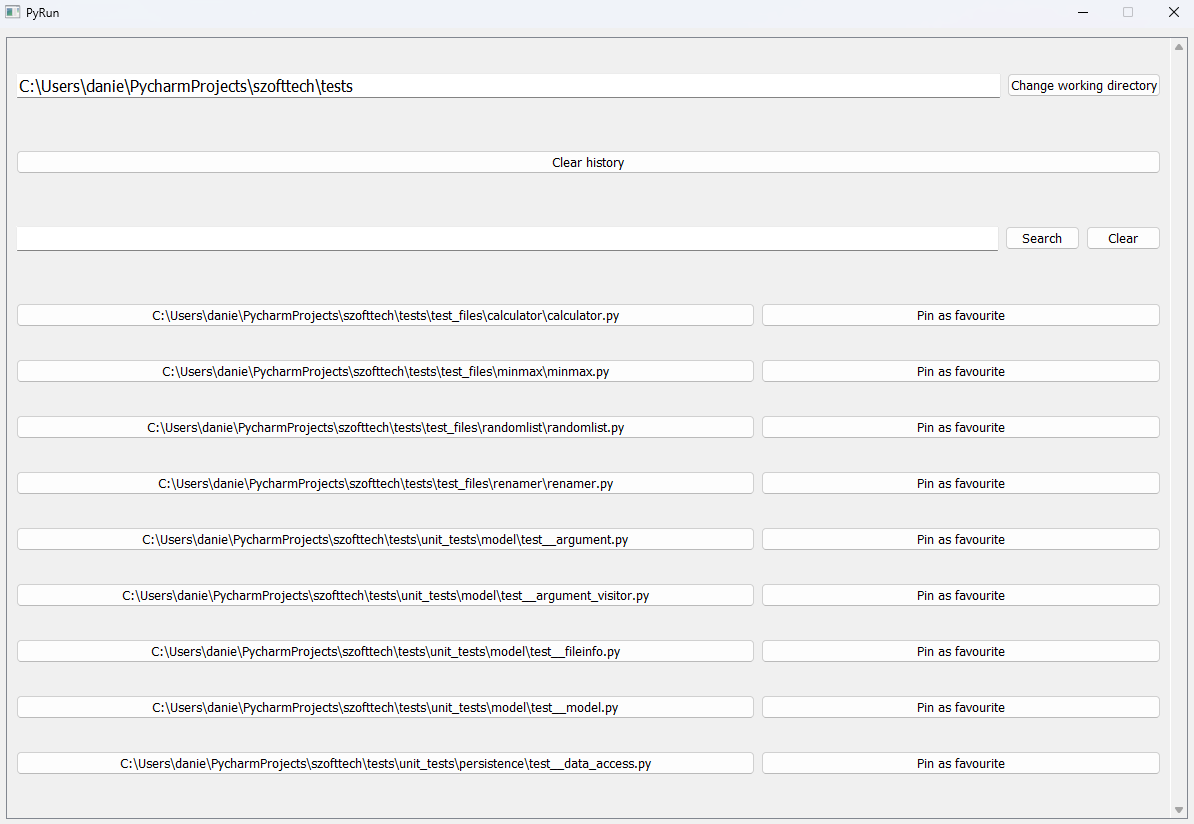
\includegraphics[width=1\linewidth]{img/main_page.png}
    \caption{Main page}
    \label{fig:enter-label}
\end{figure}

\begin{figure}[h]
    \centering
    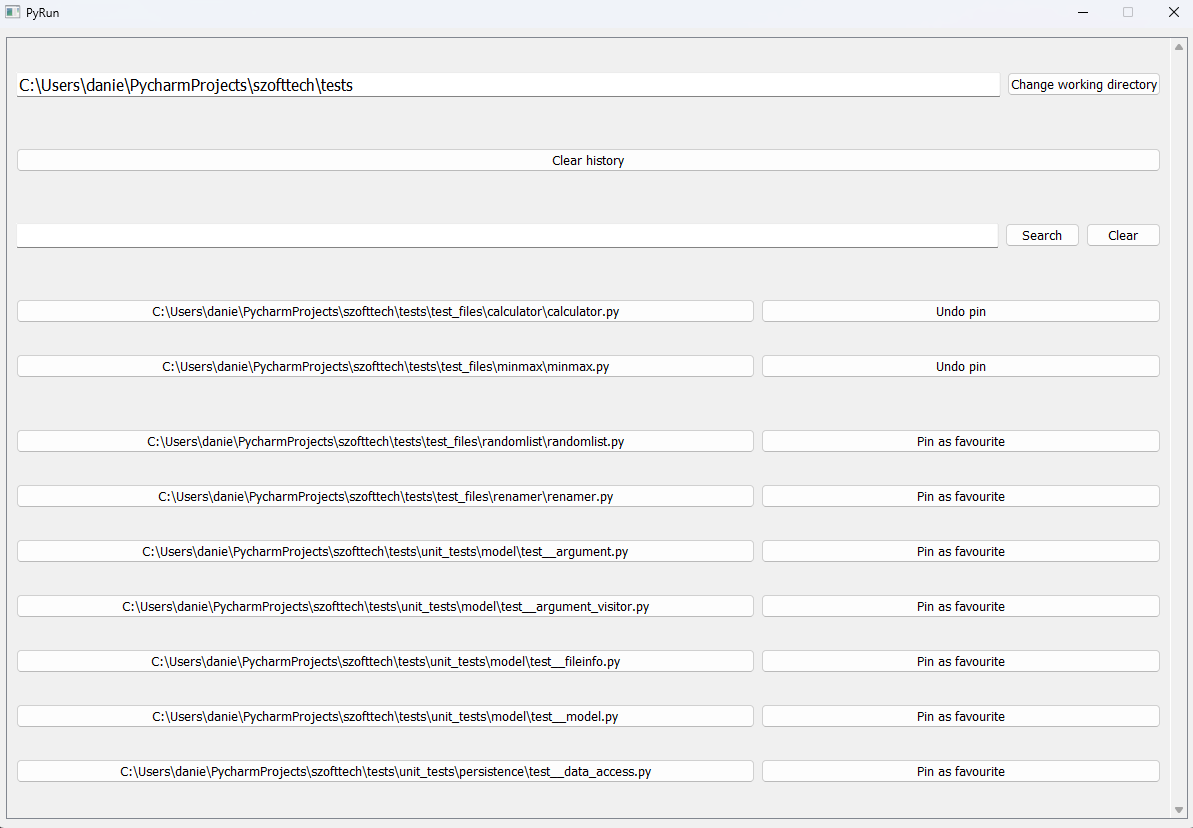
\includegraphics[width=1\linewidth]{img/pinned.png}
    \caption{Main page with pinned runnable}
    \label{fig:enter-label}
\end{figure}


\begin{figure}[h]
    \centering
    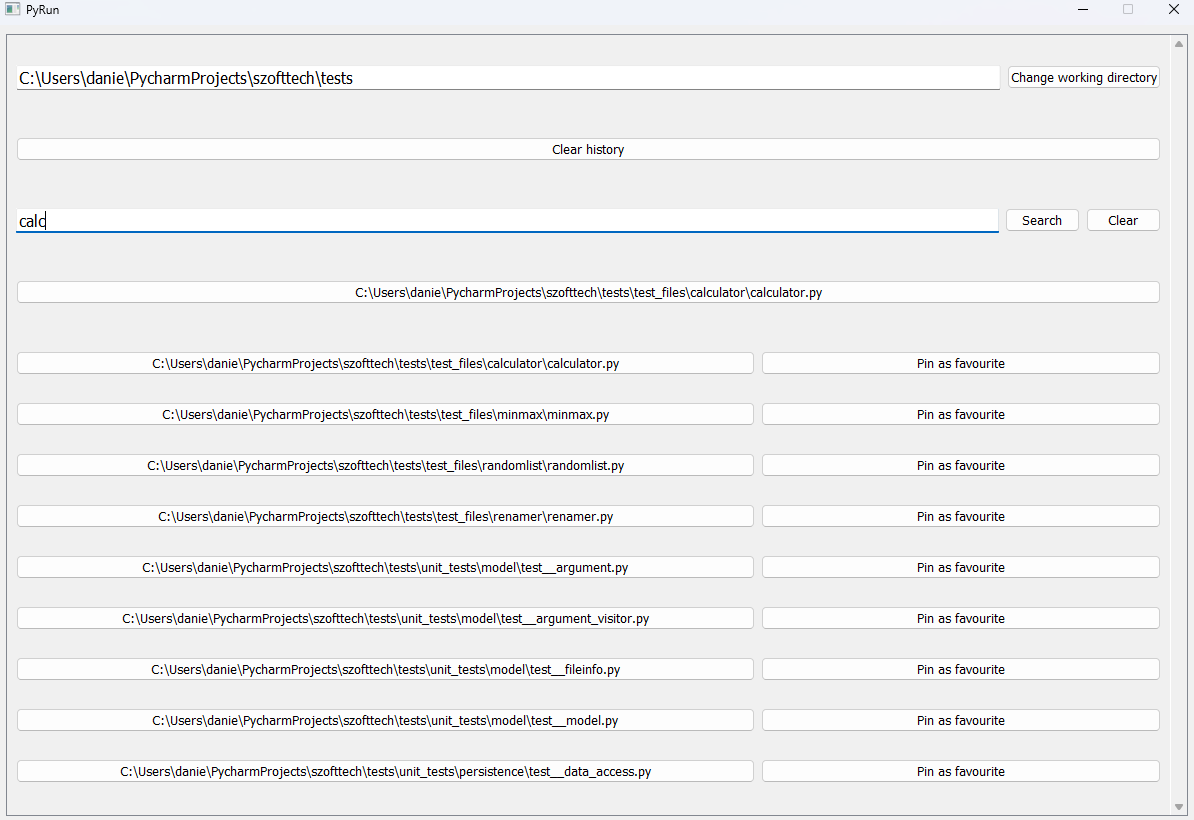
\includegraphics[width=1\linewidth]{img/search.png}
    \caption{Main page when the User searches}
    \label{fig:enter-label}
\end{figure}

\clearpage

After the User runnable pick, on the configuration page:
\begin{itemize}
    \item The User got every important information of the runnable script.
    \item The Uses are able to add values to the arguments in an input field. 
    \item The can toggle flag arguments of the runnable.
    \item If the argument contains choices, the program shows it for the User, and the User can select from them.
    \item The program saves the last configuration automatically and if the same configuration page opened again, the program loads the last argument configuration.
    \item One of the main feature of the program is that the User can execute the script.
    \item Last but not least, the User can clear the current configuration.
\end{itemize}

\begin{figure}[h]
    \centering
    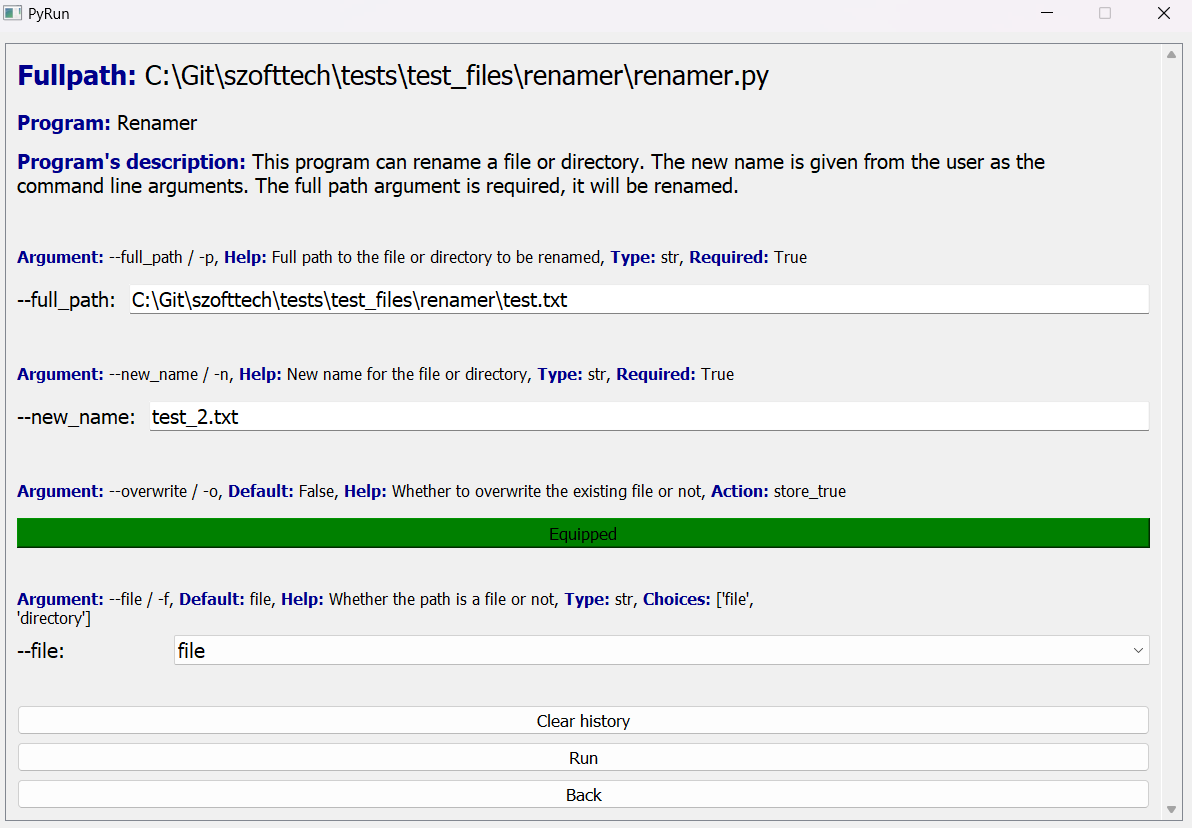
\includegraphics[width=1\linewidth]{img/config_page.png}
    \caption{Caption}
    \label{fig:enter-label}
\end{figure}

\clearpage

After running a script the Users are able to see the output of a program, or the error message, if something goes wrong.

\begin{figure}
    \centering
    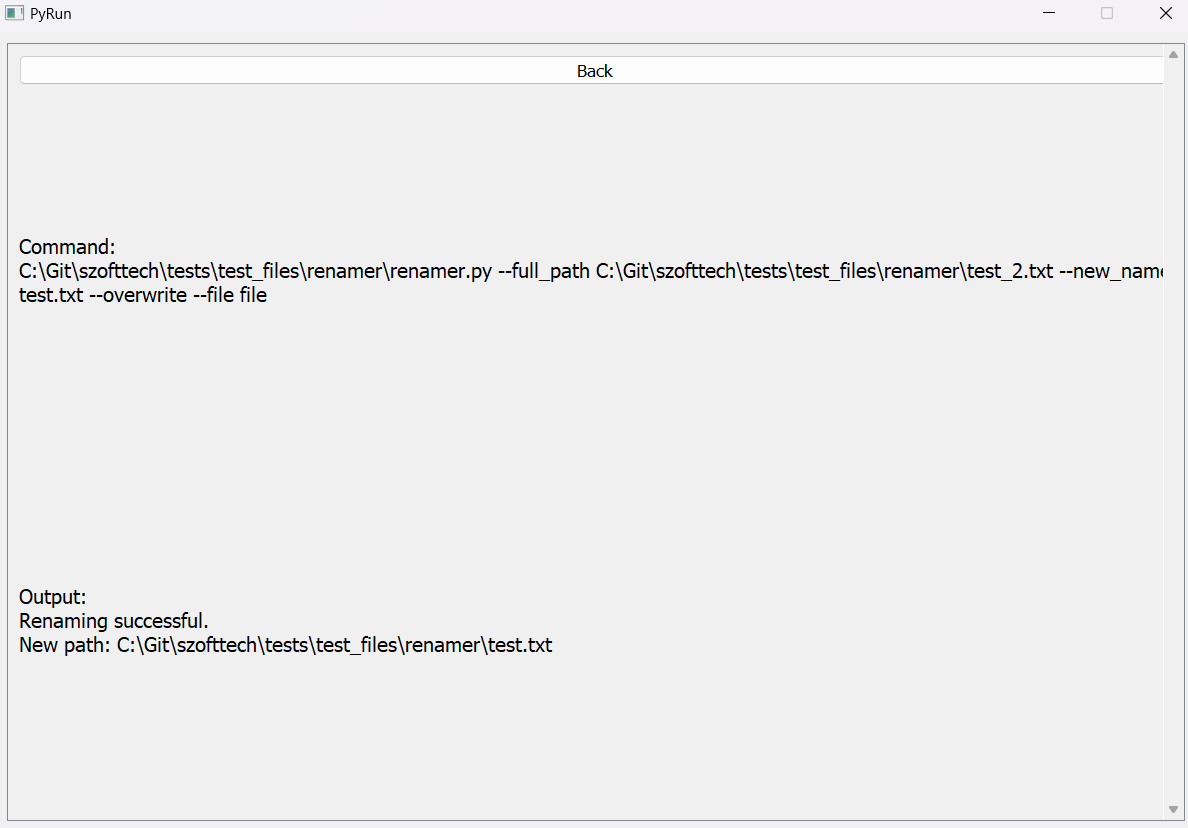
\includegraphics[width=1\linewidth]{img/runner_page.png}
    \caption{Caption}
    \label{fig:enter-label}
\end{figure}

\subsection{Conclusion}

We are pleased to confirm that all the MVP features outlined above have been successfully implemented in the program. Each point has been carefully developed and integrated, ensuring the application meets the initial goals and requirements.

\clearpage

\section{KPI goals}
We have defined the KPI in this way: \\
The KPI measures the completion rate of the core features and functionalities planned for the project.
This metric helped us objectively assess the progress and success of the project by focusing on the implementation of key deliverables that form the foundation of the system's functionality. \\
The KPI is calculated as the percentage of core features implemented out of the total planned features. In our case, these core features were clearly defined and broken down into 12 specific use cases, each representing a critical aspect of the project's functionality. These use cases were identified during the planning phase, with careful consideration of both stakeholder requirements and technical feasibility, ensuring that they accurately reflect the project's objectives. \\
At the conclusion of the implementation phase, we verified that all 12 planned use cases had been successfully developed. Therefore our KPI can be calculated as follows:
\[ \frac{implemented\ use\ cases}{planned\ use\ cases} * 100 = \frac{12}{12}*100 = 100 \]

As a result, our KPI is 100\%, and since our target was also to achieve 100\%, we can confidently state that we have successfully completed our goal. This accomplishment is a testament to the team's hard work, effective planning, and strong collaboration throughout the project lifecycle.

\end{document}